\chapter{Introduction}
\label{ch:introduction}
\graphicspath{{figures/ch_1/}}

The statistical modeling of infectious disease data is among the oldest applications of statistics, beginning with Bernoulli's work on smallpox in the 18th century \citep{Bernoulli2004}.
Today, it is an increasingly relevant application of research, due to globalization that enables diseases to spread further and faster, as well as the abundance of relevant data from electronic surveillance systems, social contact and mobility patterns from mobile phones, and genetic sequencing of pathogens.
The importance of this pursuit is apparent when reflecting on the recent COVID-19 pandemic, which resulted in millions of deaths and the largest global recession in nearly a century \citep{whocoronavirus,  zumbrun_2020}.

\section{Epidemic Surveillance Data and Its Applications}
\label{sec:epidemic_surveillance_data}
This work considers both active and passive surveillance data.

Infectious disease data differs from data used in traditional statistical applications because they are highly dependent in time and space, and are almost always partially observed \citep{held2019handbook}.
People without healthcare access or who do not exhibit disease symptoms may not seek diagnosis, leading to systematic bias and under-reporting in case counts.
Among those who seek diagnosis, their disease status may not be correctly identified, and their results may not be reported to a centralized database.
Even among those who receive correct diagnosis and whose results are reported, the precise timing of infection, transmission, and recovery are generally unknown.
These factors make statistical inference challenging.
For instance, a small outbreak with a high reporting rate may produce similar observed case counts as a large outbreak with a low reporting rate.
The situation is even more opaque for endemic diseases, where these unreported cases contribute to differing levels of immunity throughout a population.

Infectious disease surveillance data can be reported at a variety of resolutions and used for a variety of tasks.
Some methods are designed to work with detailed data from a specific, relatively small, outbreak, while others are more suitable for widespread diseases observed with less detail.
This work is primarily concerned with the latter scenario and uses passive surveillance data, which traditionally takes the form of aggregated counts of incidence data (e.g. new tests, new cases, and new deaths), counts of prevalence data (e.g. number of hospitalized patients with a disease) at some coarse demographic, spatial, and temporal resolution (e.g. stratified by age and county every week).
This and other recent advances seek to integrate other forms of data into this framework \citep{Tang2022, Rasmussen2011}.
In particular, we aim to incorporate seroprevalence studies and information derived from genetic sequencing.
These data and models are vital tools for both inference and prediction tasks.
One major goal in the inference context is nowcasting, which typically involves estimating the effective reproduction number, \( R_t \), in real time \citep{10.1093/aje/kwt133}.
This parameter is defined as the expected number of secondary cases that arise from a primary case and is influenced by factors inherent to the pathogen, as well as the environmental conditions.
For example, consider the case of a new virus variant emerging in the summer.
The new variant may be inherently more transmissible than the previously circulating strain, driving up the effective reproduction number.
Simultaneously, the warmer weather and school closures work to decrease the effective reproduction number.
Of most concern is the threshold \( R_t = 1 \).
When \( R_t < 1 \), the average primary case produces fewer than one secondary case.
If this is sustained, prevalence will decrease.
When \( R_t > 1 \), the average primary case produces more than one secondary case, leading to an exponential increase in cases.
Other inference tasks involve quantifying the effects of interventions, whether they be pharmaceutical (e.g. vaccination campaigns) or non-pharmaceutical (e.g. mask mandates).
Forecasting is concerned with anticipating future disease burden, with special attention to severe outcomes like hospitalizations and deaths \citep{10.1371/journal.pmed.1003793}.
Forecasts can combine historical data with possible future scenarios to drive public policy by answering questions like ``in the presence of a more transmissible variant, how many people do we need to vaccinate to prevent the healthcare system from being overwhelmed?"

In the next section, we provide an overview of data from these settings to motivate our methodological contributions.

\section{Motivating Examples}
\label{sec:motivating_examples}

In Chapter~\ref{ch:content_1}, we analyze data from Kalish paper, data collected from each state in the US between May and July 2020.
In Chapter~\ref{ch:content_2}, we analyze data from Orange County, California, provided to us by the Orange County Health Care Agency as well as a seroprevalence study by idk who.

\begin{figure}
    \centering
    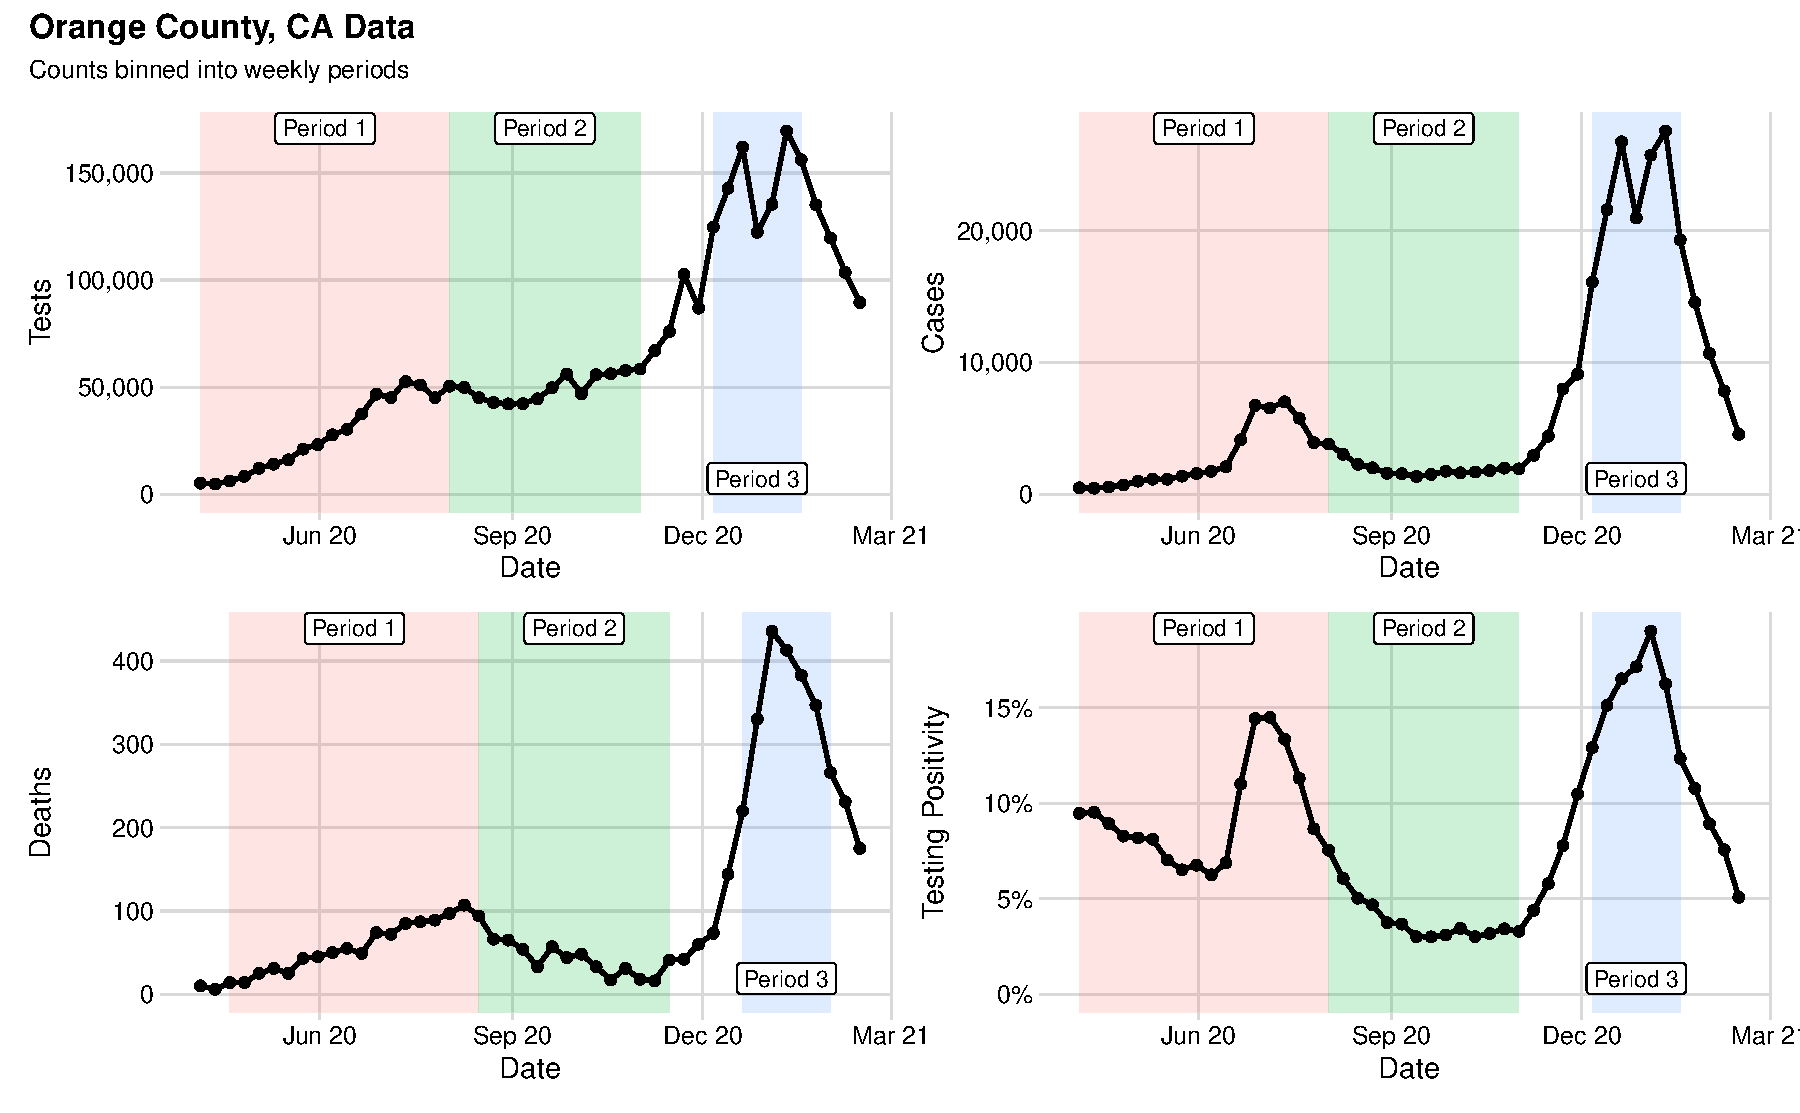
\includegraphics[width=1.0\columnwidth]{binned_data_plot}
    \caption{Caption}
    \label{ch_1:fig:binned_data_plot}
\end{figure}

Resolving the convflinct in this figure is the goal of Chapter~\ref{ch:content_2}.

In Chapter~\ref{ch:content_3}, we analyze data from tk additional California counties, provided to us by the California Department of Public Health and GISAID via outbreak package.

\section{Overview of this dissertation}
Chapter~\ref{ch:background} provides background information on areas of statistics essential to understanding the methods proposed and assessed in this dissertation.
The topics covered include mathematical models for the spread of infectious diseases, Bayesian inference and Markov chain Monte Carlo, forecast assessment, and fiducial inference.

In Chapter~\ref{ch:content_1}, we eschew the temporal complications of analyzing infectious disease data and focus on issues of sampling schemes and diagnostic test accuracy.
While there are established methods for estimating disease prevalence with associated confidence intervals for complex surveys with perfect assays and simple random sample surveys with imperfect assays, the complicated case of complex surveys with imperfect assays remains relatively unexplored.
We develop and study new methods for this setting.
The new methods use the melding method to combine gamma intervals for directly standardized rates and established adjustments for imperfect assays by estimating sensitivity and specificity.
One of the new methods appears to have at least nominal coverage in all simulated scenarios.
We compare our new methods to established methods in special cases (complex surveys with perfect
assays or simple surveys with imperfect assays).
In some simulations, our methods appear to guarantee coverage, while competing methods have much lower than nominal coverage, especially when overall prevalence is very low.
In other settings, our methods are shown to have higher than nominal coverage.
We apply our method to a seroprevalence survey of SARS-CoV-2 in undiagnosed adults in the United States between May and July 2020.

In Chapter~\ref{ch:content_2}, we turn our attention to the temporal dynamics of infectious diseases in the presence of changing policy and behavior.
Mechanistic models fit to streaming surveillance data are critical for understanding the transmission dynamics of an outbreak as it unfolds in real-time.
However, transmission model parameter estimation can be imprecise, and sometimes even impossible because surveillance data are noisy and not informative about all aspects of the mechanistic model.
To partially overcome this obstacle, Bayesian models have been proposed to integrate multiple surveillance data streams. 
We devise a modeling framework for integrating SARS-CoV-2 diagnostics test and mortality time series data, as well as seroprevalence data from cross-sectional studies, and tested the importance of individual data streams for both inference and forecasting.
Importantly, our model for incidence data accounts for changes in the total number of tests performed.
We apply our Bayesian data integration method to COVID-19 surveillance data collected in Orange County, California between March 2020 and February 2021 and find that 32--72\% of the Orange County residents experienced SARS-CoV-2 infection by mid-January, 2021.
Despite this high number of infections, our results suggest that the abrupt end of the winter surge in January 2021 was due to both behavioral changes and a high level of accumulated natural immunity.

In Chapter~\ref{ch:content_3}, we work in a similar setting as Chapter~\ref{ch:content_3}, but where the changing disease dynamics are due to novel disease variants, rather than changing policy and behavior.
Abstract tk

We conclude with a summary of our work in Chapter~\ref{ch:discussion} and discuss opportunities for future research in inference and forecasting for infectious disease data.

\label{sec:thesis_contributions}

%touch on traditional methods (SIR Model)

% This is an example using the \LaTeX{} template for UCI theses and
% dissertation documents \cite{uci-thesis-latex}. Figure
% \ref{fig:sourcecode} is just for illustration purposes, as is Table
% \ref{tab:coordinates}.

% \begin{figure}
% \begin{verbatim}
% #include <iostream>
% int main(int argc, char** argv) {
%   std::cout << "Hello World." << std::endl;
%   return 0;
% }
% \end{verbatim}
%   \caption{Example source code.}
%   \label{fig:sourcecode}
% \end{figure}

% \section{Background}

% Lorem ipsum dolor sit amet, consectetur adipisicing elit, sed do
% eiusmod tempor incididunt ut labore et dolore magna aliqua. Ut enim ad
% minim veniam, quis nostrud exercitation ullamco laboris nisi ut
% aliquip ex ea commodo consequat. Duis aute irure dolor in
% reprehenderit in voluptate velit esse cillum dolore eu fugiat nulla
% pariatur. Excepteur sint occaecat cupidatat non proident, sunt in
% culpa qui officia deserunt mollit anim id est laborum.

% \begin{table}
%   \centering
%   \begin{tabular}{|rr|r|}
%     \hline
%     $x$ & $y$ & $z$ \\
%     \hline
%     14 & 12 & -2 \\
%     0 & 33 & -25 \\
%     -3 & 11 & 22 \\
%     4 & 4 & 6 \\
%     \hline
%   \end{tabular}
%   \caption{Example coordinates.}
%   \label{tab:coordinates}
% \end{table}

% Lorem ipsum dolor sit amet, consectetur adipisicing elit, sed do
% eiusmod tempor incididunt ut labore et dolore magna aliqua. Ut enim ad
% minim veniam, quis nostrud exercitation ullamco laboris nisi ut
% aliquip ex ea commodo consequat. Duis aute irure dolor in
% reprehenderit in voluptate velit esse cillum dolore eu fugiat nulla
% pariatur. Excepteur sint occaecat cupidatat non proident, sunt in
% culpa qui officia deserunt mollit anim id est laborum.


%%% Local Variables: ***
%%% mode: latex ***
%%% TeX-master: "thesis.tex" ***
%%% End: ***
